%%%%%%%%%%%%%%%%%%%%%%%%%%%%%%%%%%%%%%%%%
% Dreuw & Deselaer's Poster
% LaTeX Template
% Version 1.0 (11/04/13)
%
% Created by:
% Philippe Dreuw and Thomas Deselaers
% http://www-i6.informatik.rwth-aachen.de/~dreuw/latexbeamerposter.php
%
% This template has been downloaded from:
% http://www.LaTeXTemplates.com
%
% License:
% CC BY-NC-SA 3.0 (http://creativecommons.org/licenses/by-nc-sa/3.0/)
%
%%%%%%%%%%%%%%%%%%%%%%%%%%%%%%%%%%%%%%%%%

%----------------------------------------------------------------------------------------
%	PACKAGES AND OTHER DOCUMENT CONFIGURATIONS
%----------------------------------------------------------------------------------------

\documentclass[final,hyperref={pdfpagelabels=false}]{beamer}

\usepackage[orientation=portrait,size=a0,scale=1.4]{beamerposter} % Use the beamerposter package for laying out the poster with a portrait orientation and an a0 paper size

\usetheme{I6pd2} % Use the I6pd2 theme supplied with this template

\usepackage[english]{babel} % English language/hyphenation

\usepackage{amsmath,amsthm,amssymb,latexsym} % For including math equations, theorems, symbols, etc

%\usepackage{times}\usefonttheme{professionalfonts}  % Uncomment to use Times as the main font
%\usefonttheme[onlymath]{serif} % Uncomment to use a Serif font within math environments

\boldmath % Use bold for everything within the math environment

\usepackage{booktabs} % Top and bottom rules for tables

\graphicspath{{figures/}} % Location of the graphics files

\usecaptiontemplate{\small\structure{\insertcaptionname~\insertcaptionnumber: }\insertcaption} % A fix for figure numbering

%----------------------------------------------------------------------------------------
%	TITLE SECTION 
%----------------------------------------------------------------------------------------

\title{\huge The Effect of Lake Connectivity on Phosphorus Retention in Lakes} % Poster title

\author{Joseph Stachelek} % Author(s)

\institute{Department of Fisheries and Wildlife, Michigan State University, MI, USA} % Institution(s)

%----------------------------------------------------------------------------------------
%	FOOTER TEXT
%----------------------------------------------------------------------------------------

\newcommand{\leftfoot}{} % Left footer text

\newcommand{\rightfoot}{stachel2@msu.edu} % Right footer text

%----------------------------------------------------------------------------------------

\begin{document}

\addtobeamertemplate{block end}{}{\vspace*{2ex}} % White space under blocks

\begin{frame}[t] % The whole poster is enclosed in one beamer frame

\begin{columns}[t] % The whole poster consists of two major columns, each of which can be subdivided further with another \begin{columns} block - the [t] argument aligns each column's content to the top

\begin{column}{.02\textwidth}\end{column} % Empty spacer column

\begin{column}{.465\textwidth} % The first column

%----------------------------------------------------------------------------------------
%	INTRODUCTION
%----------------------------------------------------------------------------------------
            
\begin{block}{Introduction}

\begin{itemize}
\item A comprehensive understanding of phosphorus (P) cycling is neccessary to predict P concentrations among many different lakes types and to better manage the risk of eutrophication from excess nutrient loading.
\item P retention is a desirable metric for assessing eutrophication risk because it is a unitless measure that can be easily compared among different lake types irrespective of their baseline P concentrations or total P inputs.
\item In the absence of direct measurement, P retention is typically modelled as a function of a given lake's volume-weighted hydrologic flux (or its inverse, \alert{residence time}).
\end{itemize}

\end{block}

%----------------------------------------------------------------------------------------
%	Research Questions
%----------------------------------------------------------------------------------------
{
\setbeamercolor{block title}{fg=black,bg=orange!70} % Change the block title color
\setbeamercolor{block body}{bg=white}
\begin{block}{Research Questions}

\begin{figure}
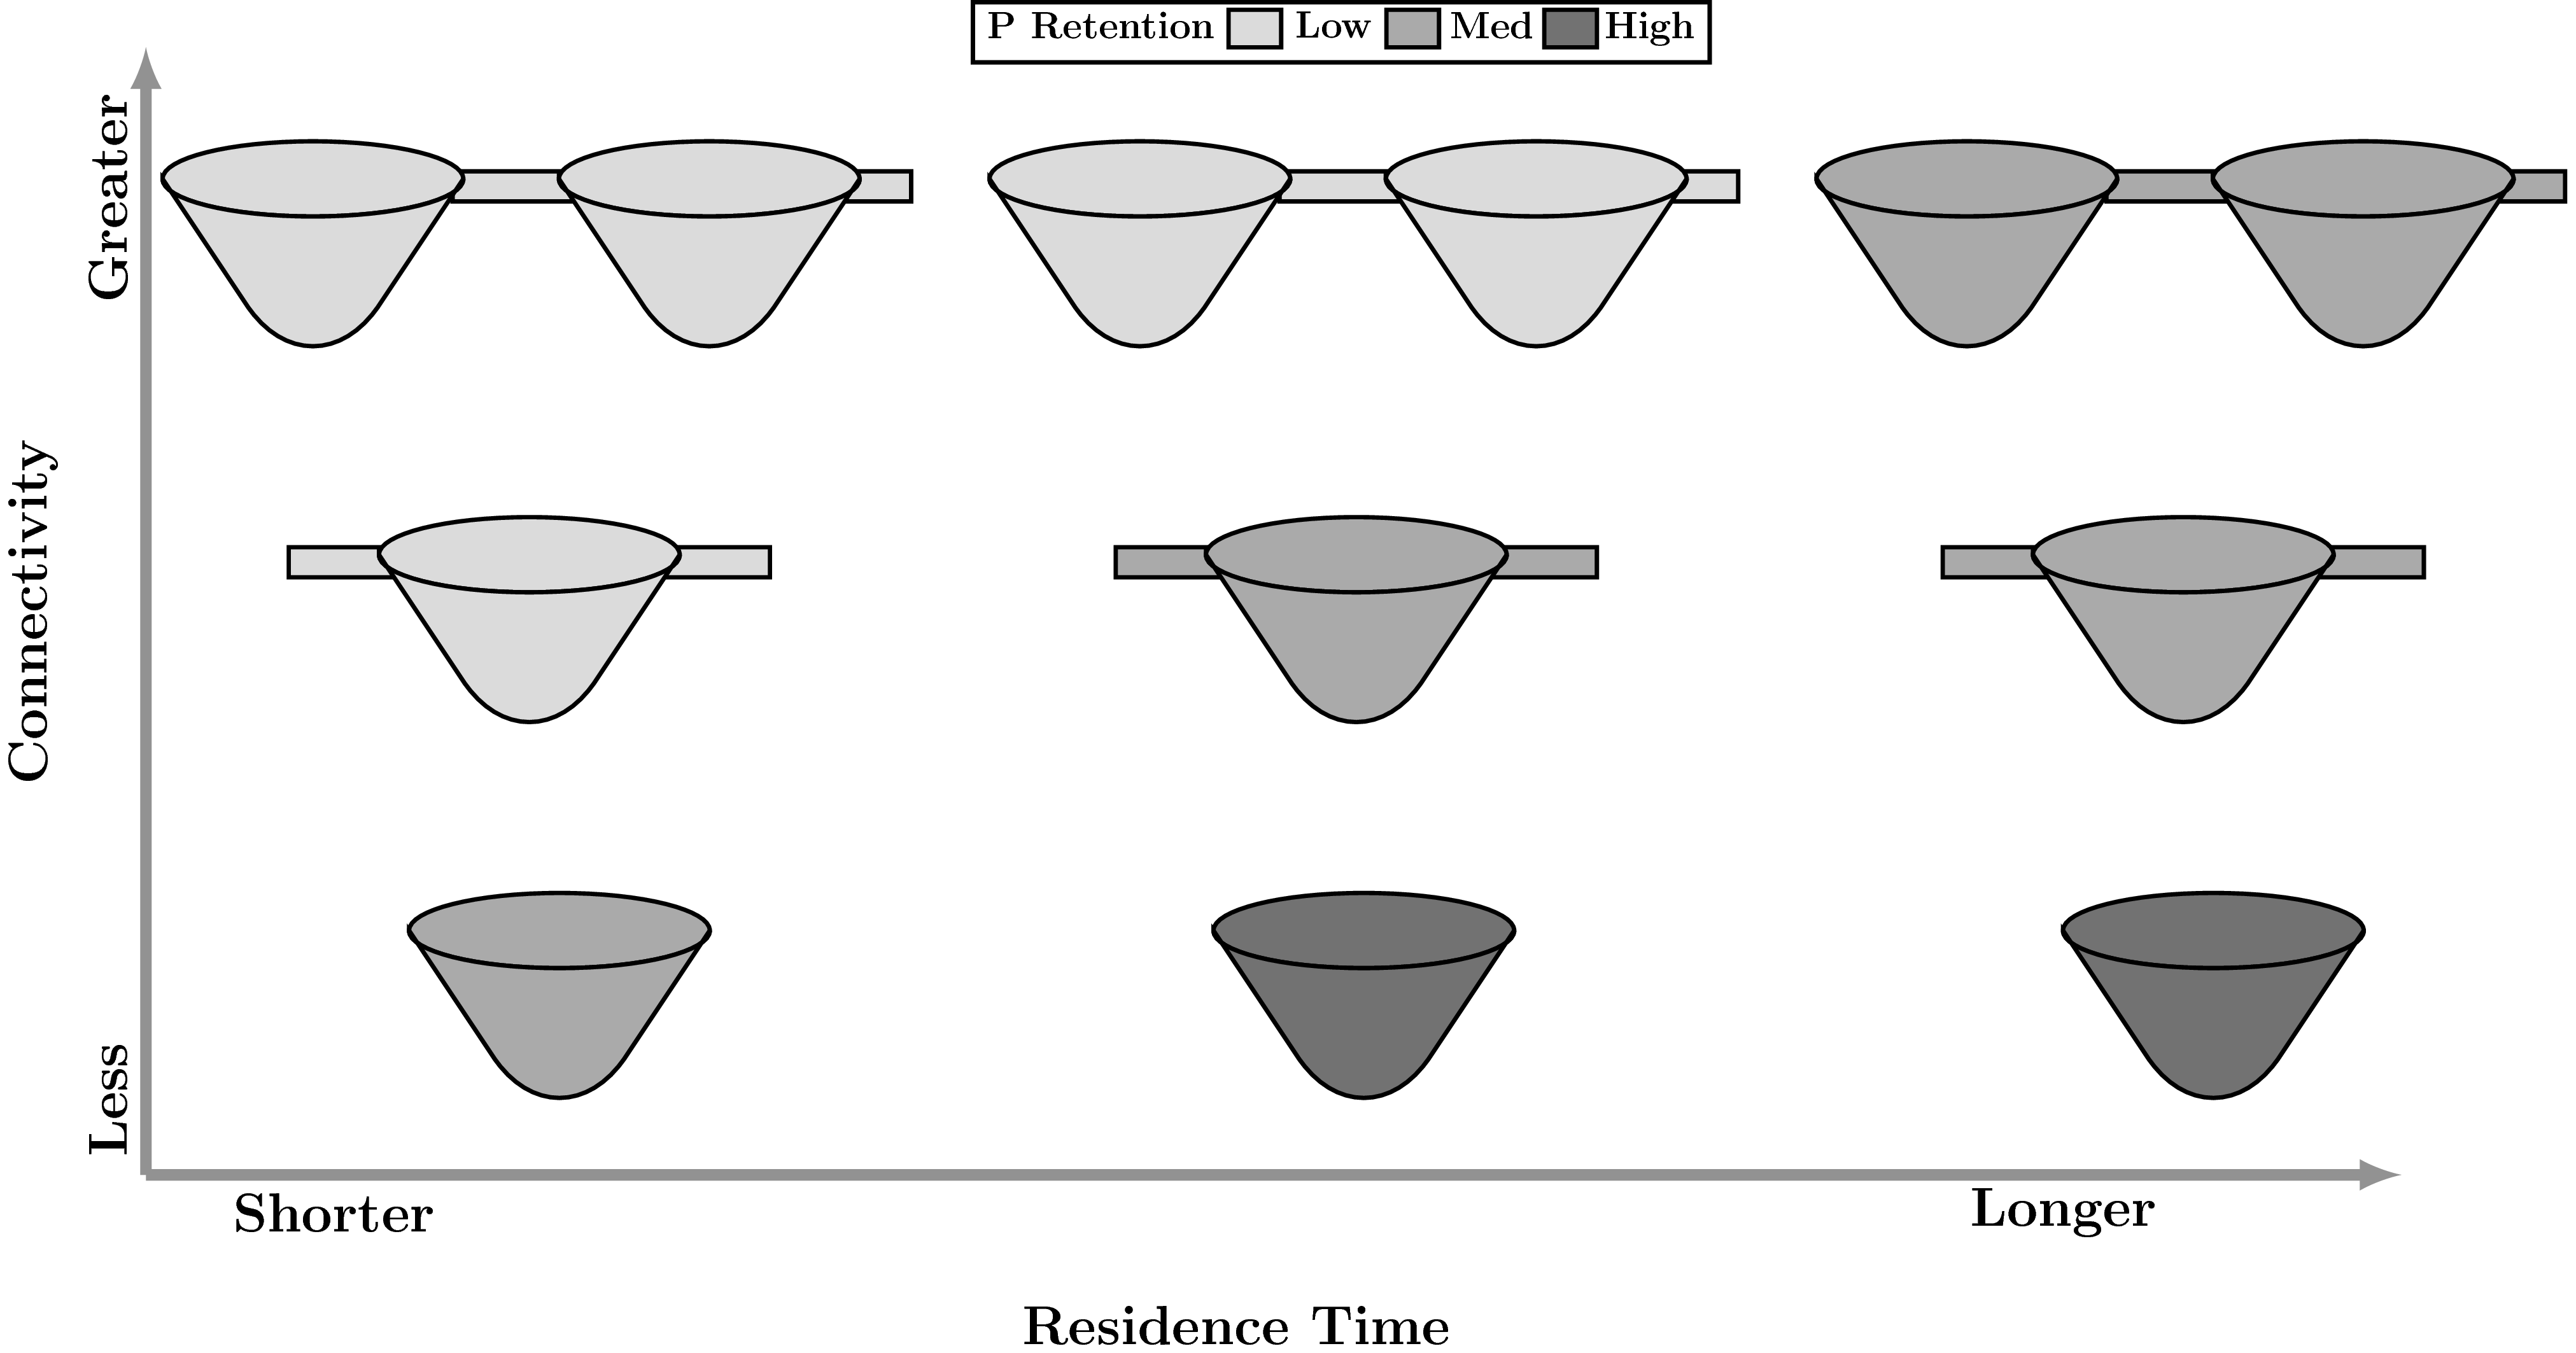
\includegraphics[width=\linewidth]{conny_framework.png}
\end{figure}

\begin{enumerate} \large 
\item \textbf{In lakes with equal residence times, do more well-connected lakes retain less P than lower connectivity lakes?}
\item \textbf{Is the effect of connectivity on P retention more prominent in lakes with intermediate residence times?}
\end{enumerate}

\end{block}
}

%----------------------------------------------------------------------------------------
%	METHODS
%----------------------------------------------------------------------------------------
\begin{block}{Methods}

\begin{columns} % Subdivide the first main column
\begin{column}{\textwidth} % The first subdivided column within the first main column
\begin{itemize}
\item Lakes were sampled on a monthly basis for a one year period in one of 197*, 197*, 197*, or 197*.
\item P loads were estimated as the sum of the loads contributed by incoming tributaries.
\item Retention time was computed on the basis of concurrent USGS gage measurements normalized to estimate a mean flow for each month in an average year.
\item P retention was computed using a modification of the Vollenweider equations (see under flap).
\item Proin ut vestibulum augue.
\begin{itemize}
\item Donec dapibus sagittis neque eu ultrices.
\end{itemize}
\end{itemize}
\end{column}

% \begin{column}{.43\textwidth} % The second subdivided column within the first main column
% \centering
% \begin{figure}
% 
\includegraphics[width=0.8\linewidth]{placeholder.jpg}
% \caption{Figure caption}
% \end{figure}
% \end{column}
\end{columns} % End of the subdivision

\begin{itemize}
\item Curabitur sapien ligula, faucibus in feugiat quis, vestibulum a turpis.
\begin{itemize}
\item Phasellus quis nunc neque.
\end{itemize}
\end{itemize}

\begin{itemize}
\item Maecenas Ultricies Feugiat Velit Non Mattis.
\begin{itemize}
\item Duis ante erat, bibendum nec tempus nec, interdum quis est. Nulla at mollis tortor. Phasellus quis leo dolor, aliquam laoreet orci $X$ Donec dapibus sagittis neque eu nec, interdum quis est. $Y_n, n=1,\cdots,N$ ndum nec tempus nec, interd
\begin{align*}
X \rightarrow r(X) & = \arg \max_{c} \Big\{ \max_n \big\{ \sum_{x_i \in X} \delta(x_i,Y_{n,c})\big\} \Big\} 
\end{align*}
\item Cras faucibus scelerisque cursus. Proin ut vestibulum augue. $\delta(x_i,Y_{n,c})$
\end{itemize}
\item Fusce tempus arcu id ligula varius dictum. Donec ut nisl dui.
\end{itemize}

\end{block}

%----------------------------------------------------------------------------------------

\end{column} % End of the first column

\begin{column}{.03\textwidth}\end{column} % Empty spacer column
 
\begin{column}{.465\textwidth} % The second column

%----------------------------------------------------------------------------------------
%	RESULTS
%----------------------------------------------------------------------------------------

\begin{block}{Results: Table}

\begin{itemize}
\item Ased Aliquet Luctus Lectus
\end{itemize}

\begin{table}
\begin{tabular}{l l l}
\toprule
\textbf{Treatments} & \textbf{Response 1} & \textbf{Response 2}\\
\midrule
Treatment 1 & 0.0003262 & 0.562 \\
Treatment 2 & 0.0015681 & 0.910 \\
Treatment 3 & 0.0009271 & 0.296 \\
\bottomrule
\end{tabular}
\caption{Table caption}
\end{table}

\begin{itemize}
\item Sollicitudin Vel Orci
\item Maecenas Ultricies Feugiat Velit Non Mattis.
\end{itemize}

\begin{table}
\begin{tabular}{l l l}
\toprule
\textbf{Treatments} & \textbf{Response 1} & \textbf{Response 2}\\
\midrule
Treatment 1 & 0.0003262 & 0.562 \\
Treatment 2 & 0.0015681 & 0.910 \\
Treatment 3 & 0.0009271 & 0.296 \\
\bottomrule
\end{tabular}
\caption{Table caption}
\end{table}
     
\end{block}

%------------------------------------------------

%----------------------------------------------------------------------------------------
%	CONCLUSION
%----------------------------------------------------------------------------------------

\begin{block}{Conclusion}

\begin{itemize}
\item Opet \alert{volutpat} ligula. Duis semper lorem eget dui dignissim porttitor. Nulla facilisi. In ullamcorper lorem quis dolor iaculis nec egestas enim ultricies. Cras ut mauris elit, ut lacinia dui. Proin in ante et libero hendrerit iaculis.
\end{itemize}

\end{block}

%----------------------------------------------------------------------------------------
%	REFERENCES
%----------------------------------------------------------------------------------------

\begin{block}{References}
        
\nocite{*} % Insert publications even if they are not cited in the poster
\small{\bibliographystyle{unsrt}
\bibliography{sample}}

\end{block}

%----------------------------------------------------------------------------------------
%	CONTACT INFORMATION
%----------------------------------------------------------------------------------------

% \setbeamercolor{block title}{fg=black,bg=orange!70} % Change the block title color

\begin{block}{Contact Information}

\begin{itemize}
\item Web: \href{http://jsta.rbind.io}{http://jsta.rbind.io}
\item Email: \href{mailto:stachel2@msu.edu}{stachel2@msu.edu}
\end{itemize}

\end{block}

%----------------------------------------------------------------------------------------

\end{column} % End of the second column

\begin{column}{.015\textwidth}\end{column} % Empty spacer column

\end{columns} % End of all the columns in the poster

\end{frame} % End of the enclosing frame

\end{document}